\documentclass[a4paper,10pt]{article}
%A Few Useful Packages
\usepackage{marvosym}
\usepackage{fontspec} 					%for loading fonts
\usepackage{xunicode,xltxtra,url,parskip} 	%other packages for formatting
\RequirePackage{color,graphicx}
\usepackage[usenames,dvipsnames]{xcolor}
\usepackage[big]{layaureo} 				%better formatting of the A4 page
% an alternative to Layaureo can be ** \usepackage{fullpage} **
\usepackage{supertabular} 				%for Grades
\usepackage{titlesec}					%custom \section
%Setup hyperref package, and colours for links
\usepackage{hyperref}
\usepackage{wrapfig}
\usepackage[export]{adjustbox}
\definecolor{linkcolour}{rgb}{0,0.2,0.6}
\hypersetup{colorlinks,breaklinks,urlcolor=linkcolour, linkcolor=linkcolour}

%% Page sizes
\setlength{\textwidth}{0.92\paperwidth}
\setlength{\textheight}{720pt}
\setlength{\hoffset}{-70pt}
\setlength{\voffset}{-50pt}

%% Change subscection macro
\renewcommand\thesubsection{}

%% Fonts
\defaultfontfeatures{Mapping=tex-text}
%%% modified for Karol Kozioł for ShareLaTeX use
\setmainfont[
    SmallCapsFont = Fontin-SmallCaps.otf,
    BoldFont = Fontin-Bold.otf,
    ItalicFont = Fontin-Italic.otf
]
{Fontin.otf}

%CV Sections inspired by: 
%http://stefano.italians.nl/archives/26
\titleformat{\section}{\Large\scshape\raggedright}{}{0em}{}[\titlerule]
\titlespacing{\section}{0pt}{3pt}{3pt}

%Tweak a bit the top margin
%\addtolength{\voffset}{-1.3cm}

%Italian hyphenation for the word: ''corporations''
\hyphenation{im-pre-se}

%-------------WATERMARK TEST [**not part of a CV**]---------------
\usepackage[absolute]{textpos}

%\setlength{\TPHorizModule}{30mm}
%\setlength{\TPVertModule}{\TPHorizModule}
%\textblockorigin{2mm}{0.65\paperheight}
%\setlength{\parindent}{0pt}
%\usepackage[printwatermark]{xwatermark}
%\usepackage{xcolor}
%\usepackage{graphicx}
%\usepackage{lipsum}
%\newwatermark[allpages,color=red!50,angle=45,scale=1,xpos=-85,ypos=125]{DRAFT}
%--------------------BEGIN DOCUMENT----------------------

\begin{document}
\pagestyle{empty} % non-numbered pages

%--------------------TITLE-------------
\par{	
    
    \begin{wrapfigure}{!tr}{0.20\textwidth}
    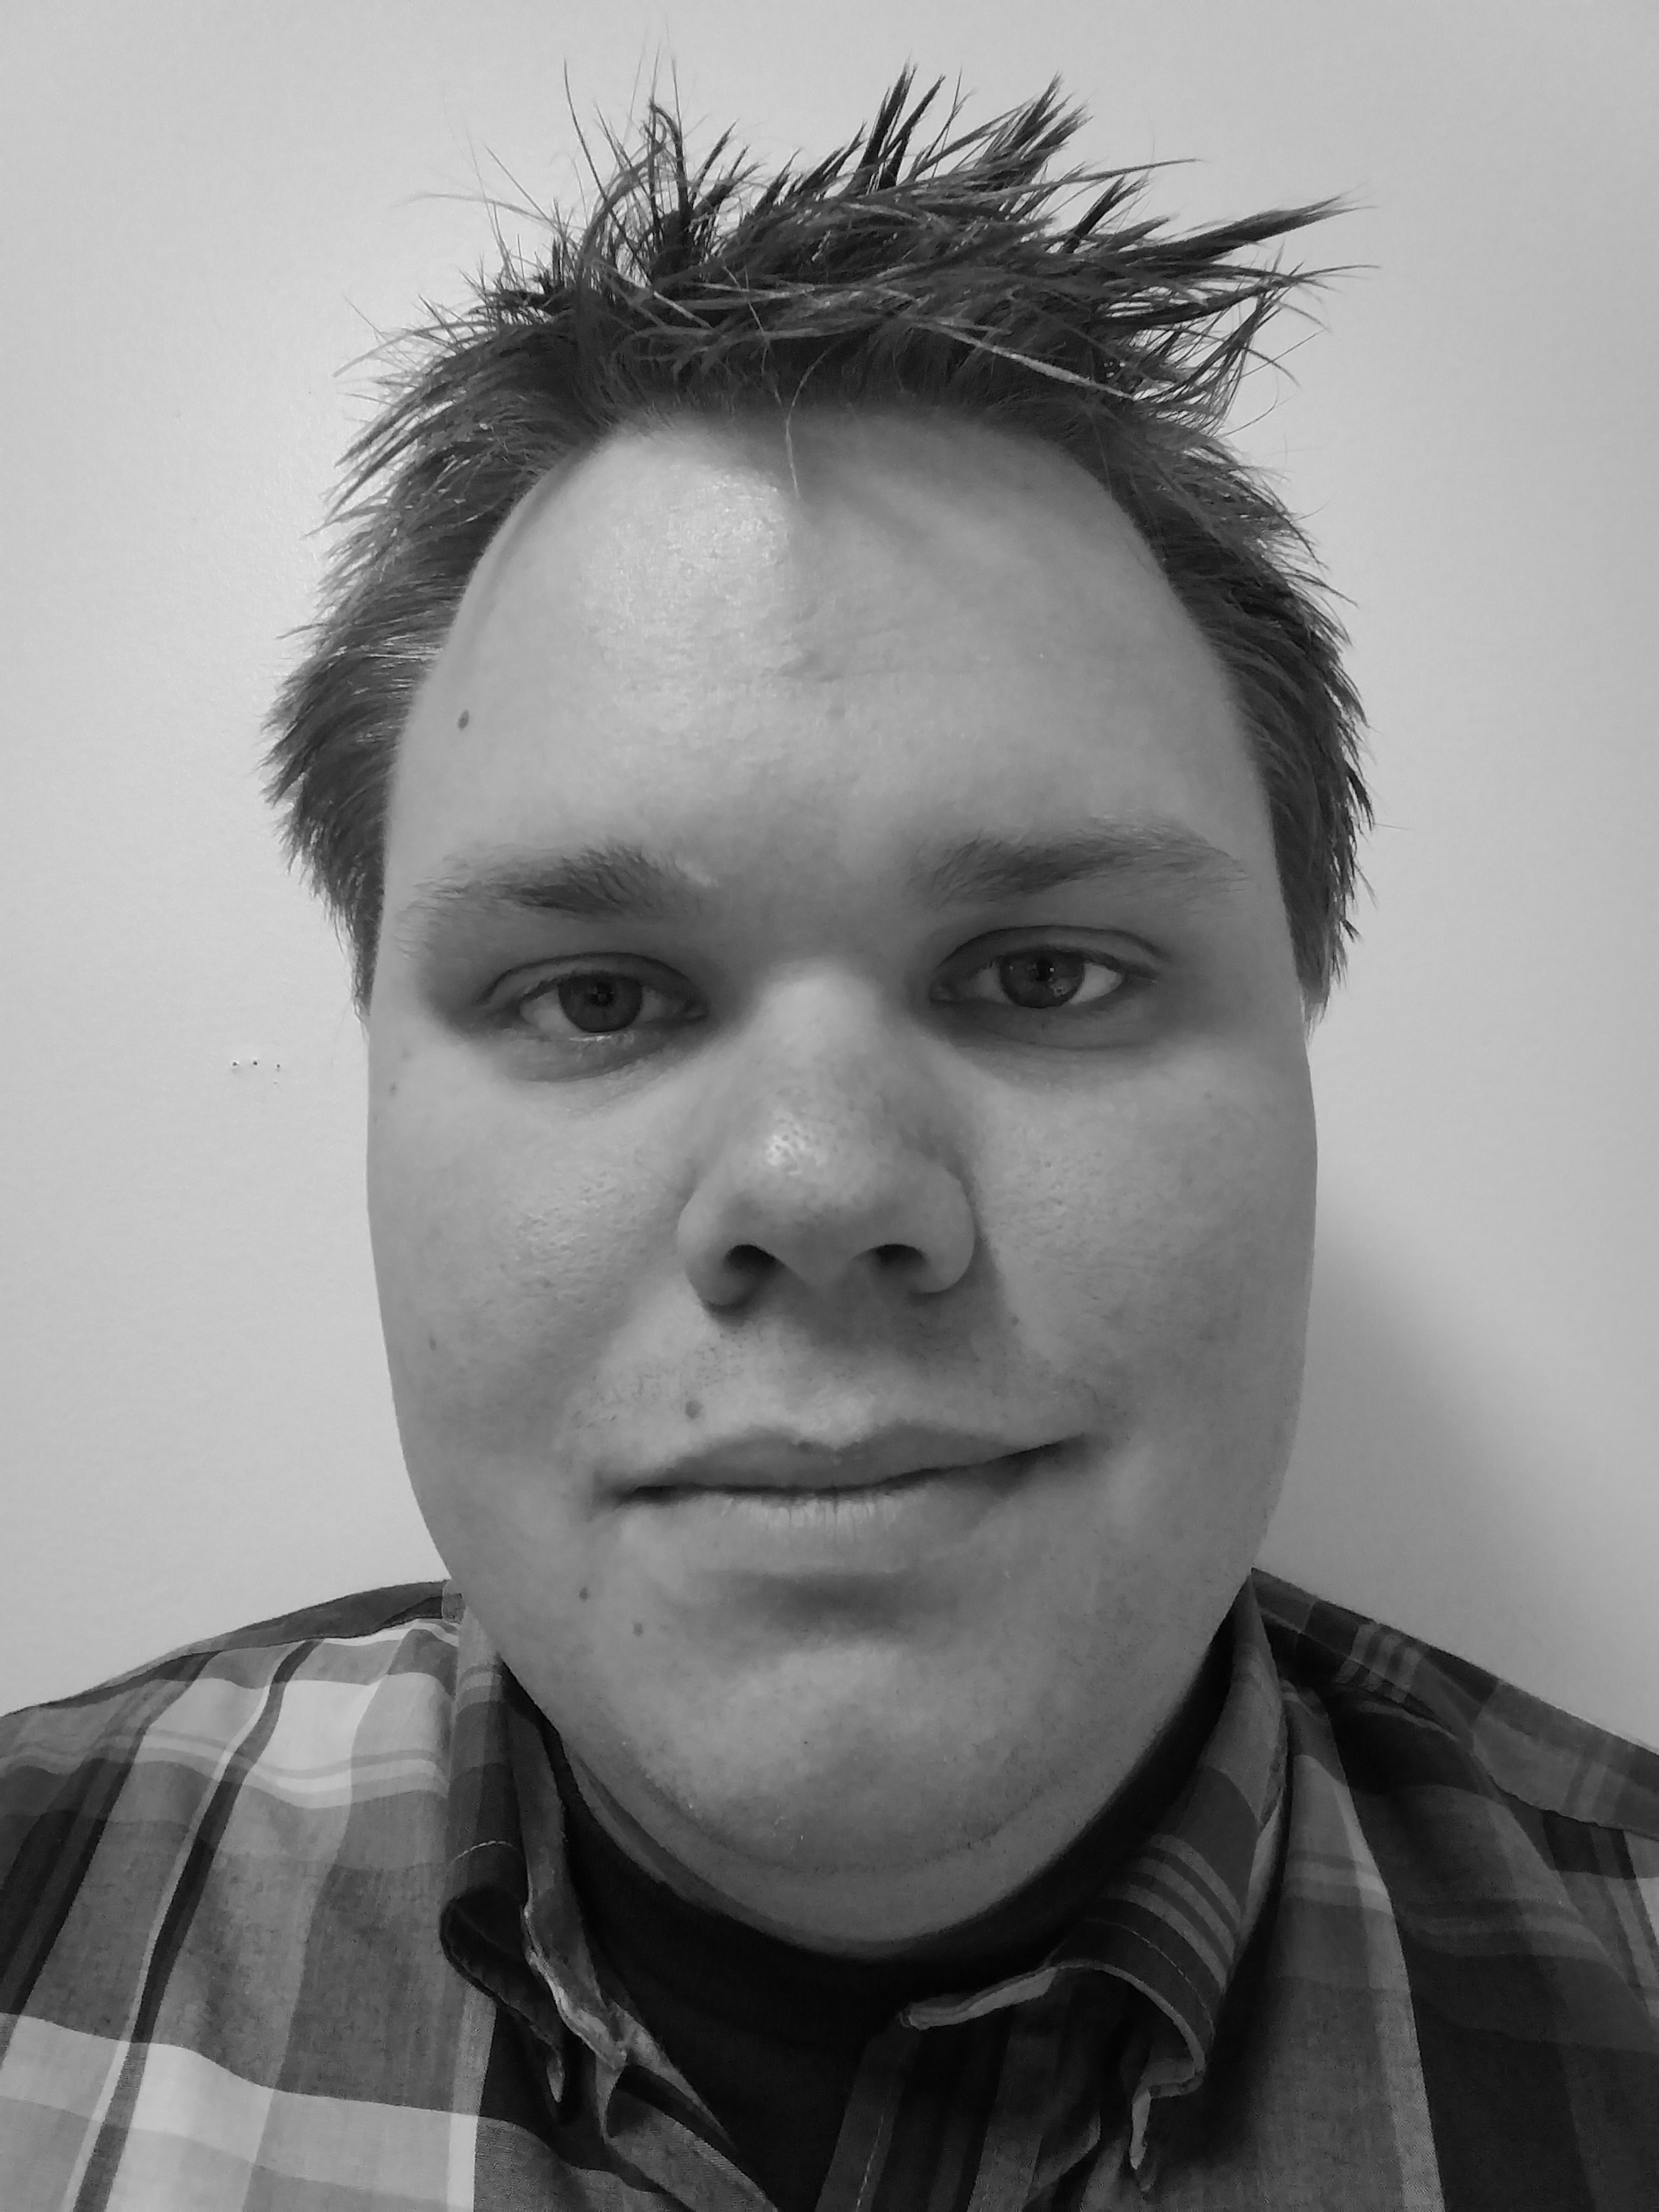
\includegraphics[scale=0.04]{Grayscale.pdf}
    \end{wrapfigure}
    
    %\Huge Rasmus \textsc{Tilljander}
    \Huge Consultant Profile
    
	\bigskip
\par}

%--------------------SECTIONS-----------------------------------

%%%
\begin{tabular}{rl}
    \textsc{} &    \\
    \textsc{Year of Birth:} &   1991   \\
    \textsc{Citizenship:}   &   Swedish \\ 
%    \textsc{Address:}   & Valhallavägen 4B, 37140 , Karlskrona, Sweden \\
    \textsc{Languages:}  & Swedish (Native), English (Fluent) \\
    \textsc{Contact:}   & 07xx-xxxxx \\
%    \textsc{Phone:}     & +46 76 00 66 242\\
%    \textsc{email:}     & tilljander.rasmus@gmail.com\\
%    \textsc{Github:}  & \url{https://github.com/Meraz}\\
%    \textsc{linkedin:}  & \url{https://se.linkedin.com/in/rasmus-tilljander-62830052}
\end{tabular}

%%%
\section{Summary}
Rasmus is a student of knowledge with genuine curiosity regarding the essential workings of the world. With an open mind he adopts the philosophy that one can always improve oneself and that each day contains opportunities that has to be seized. Due to the characteristic of software development it demands a mix of social, logical, and artistic aspects in order to excel
in. This is why Rasmus has chosen software development as his primary field of interest. As a natural approach he chose an academic road which had a low-level foundation in terms of programming but still explored areas such as visualisation and UX. Which is why C/C++ augmented with higher lever languages is the tools of his choice.

Rasmus excels at planning and organizing his surroundings and because of that he often finds himself in a position to
coordinate others, something he does well. However, as a personality trait Rasmus believes that a person never can be
completely perfect, as a results he always aims to improve himself by an iterative process where he reflects on his own
actions and the actions of others. By combining his skill in organization with self evaluation he tries to identify and
prevent pitfalls and problems before they occur.

%%%
\section{Competences)}
Expert Knowledge(5), Advanced Knowledge(4), Intermediate Knowledge(3), Basic Knowledge(2), Beginners Knowledge(1)

\begin{tabular}{rl}
Programming languages:&
C++(4),
Assembler (IA-32)(3),
C(3),
C\#(3),
HLSL(3),
Java(3),
LateX(3),
SQL(3),
XML(3),
HTML(2),\\&
Javascript(2),
LUA(2),
PHP(2),
Python(2),
Scala(2),
Matlab(1),
YAML(1)\\

Development Tools:&
CMake(4),
Bash(3),
CLion(3),
Gerrit(3),
Gradle(3),
IntelliJ(3),
Jenkins(3),
Jira(3),
Visual Studio(3),\\&
Tomcat(3),
Unity3D(3),
Apache(2),
Clang(2),
Eclipse(2),
GNU toolchain(2),
JBoss(2),
Vagrant(2),\\&
Windows Batch Script(2),
Confluence(1),
Lint(1),
Maven(1),
Powershell(1)\\

Libs and Platforms:&
Android SDK(3),
DirectX(3),
Google Test(3),
POSIX Threads(3),
STL(3),
Android NDK(2),
Boost(2),\\&
Mockito(2),
MPI(2),
OpenGL(2),
SDL(2),
Spring(2),
Angular(1),
Google Mock(1),
NodeJS(1),\\&
Wordpress(1)\\

Operating System:&
Linux(4),
Windows(4),
Unix(2),
Mac OS X(1)\\

Development Methods:&
Agile(3),
Scrum(3),
Kanban(2),
TDD(2),
CI(2),
Lean(1)\\

Databases:&
MySQL(3),
SQlite(2)\\

Version Control:&
Git(4),
svn(1)\\

Protocols and Formats:&
MQTT(2),
REST(2)\\

Other software:&
SSH(3),
cURL(2),
Office Word(2)\\
\end{tabular}

%%%
\section{Work experience}

\textbf{Consulting Software Engineer} 2017-02 - Present \\
\begin{tabular}{rl}
Employer:& ICTech\\
Assignment:& CPAC AB (2017-02 - 2017-06)
\end{tabular}\\

\textbf{Consulting Software Engineer} 2014-09 - 2017-01 \\
\begin{tabular}{rl}
Employer:& HiQ Karlskrona AB\\
(2016-04 - 2014-01):& Ericsson AB at 100\%. Rasmus were assigned multiple PoC projects and helped to create and stabilize\\& new teams as a scrummaster, lead developer, mentor, or teamleader, depending on the requirements\\& of the team. \\
(2014-09 - 2014-12):& Ericsson AB at 100\% which started as a summer intership but was continued. Rasmus had the role\\& as developer first 2-3 months but stepped up as scrummaster and teamleader after that. \\
(2014-09 - 2014-12):& Ericsson AB at 25\% with two other students where Rasmus found him self in the role as teamleader.\\

\end{tabular}\\

%%%
\section{Education}
\textbf{Blekinge Institute of Technology} 2010-09-01 - 2016-03-31\\
\begin{tabular}{rl}
Degree:&  Master of Engineering Science in Game and Software Engineering\\
Thesis:& Combining Regional Time Stepping With Two-Scale PCISPH Method\\
Notable project:& During a 20 week long project, where I acted as scrummaster, we were tasked to build  a game engine\\& and associated game from scratch in C++ using DirectX, PhysX, FMod, SDL and Winsock.
\end{tabular}\\

%%%
\section{Interests}
During his spare time Rasmus enjoys to use the computer for computer games, researching and testing new libraries, tools, frameworks, and languages. He also appreciates gamejams whenever possible and occasionally spends his time on a wargame. A special interest for Rasmus is C++ and keeping up to date with new techniques and changes for the language. Outside the digital world Rasmus enjoy cooking, magic the gathering, craft beer, and traveling. He is currently casually looking into the craftsmanship of wood carving as a hobby.

\end{document}